%****************************************************************************************************************************************
% File: shared-ontology.tex
%
% This file is automatically generated. Please do not edit!
%****************************************************************************************************************************************
\section{Ontology Overview}

The shared ontology defines concepts that do not specifically pertain to the CPS and neither to the MPM domain, but that are required by one of these domains or both. It is a place to define concepts reusable by all the ontologies developed in this effort. The classes and properties provided in this ontology may be refined by other ontologies of the framework to provide specialized definitions for more specific domains. 

The shared ontology is divided into five domains for capturing concepts related to the \uidxp{linguistic}, \uidxp{workflow}, \uidxp{project management},  \uidxp{architecture} and  \uidxp{paradigm} domains. When applicable, the classes of these domains were based on well-known standards and other de-facto standard works. 
Note that these domains are not disjoint so that a class may appear under several domain concept classes.

Figure \ref{fig:shared_ontology_overview} shows an overview of the shared ontology. The details of each concept are
provided in the following subsections.

\begin{figure}[!htb]
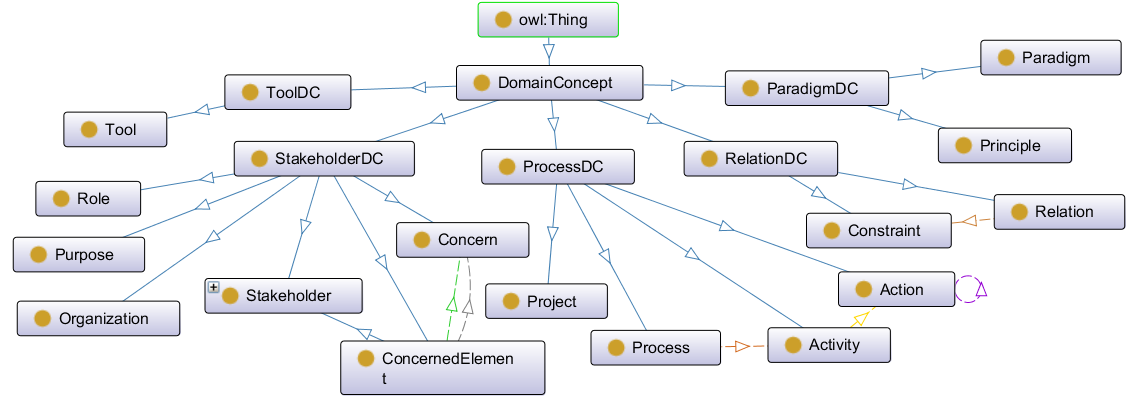
\includegraphics[width=\textwidth]{figures/shared_ontology_overview.png}
\caption{Overview of the shared ontology}
\label{fig:shared_ontology_overview}
\end{figure}

\section{DomainConcept (Domain Concepts)}
\label{sec:shared:classes}

This class groups all domain concepts of the MPM4CPS ontologies. It is further divided into  subclasses for the different sub-domains of the MPM4CPS ontologies. The classes for these sub-domains can be identified from their DC (Domain Concept) suffix. 
These sub-domain classes allow organizing the ontology into specific domains thus facilitating the navigation across the many concepts of the MPM4CPS ontologies. Note that the sub-domain classes are not disjoint from each other so that a class may belong to several sub-domain concepts.

\subsection{ArchitectureDC (Architecture Domain Concepts)}
\label{subsecDC:ArchitectureDC}

This class groups concepts that are related to the \uidxp{architecture} domain. These concepts were initially inspired from the well-known ISO/IEC/ IEEE 42010 standard and its adaptation by \cite{Broman2012}. 

The architecture is extremely vast and only a minimal subset from its concepts has been considered and adapted for the MPM4CPS sub-domains (see figure~2 of \cite{Hilliard2012}).

\subsubsection{Architecture}
\label{subsubsecC:Architecture}
\didx{Architecture}

\todoAuthors{Provide ``rdfs:comment'' annotation in ontology}

\textbf{Subclass of}
\begin{itemize}
	\item \textbf{ArchitectureDC} (see section \ref{subsecDC:ArchitectureDC})
\end{itemize}






\subsubsection{ArchitectureDescription}
\label{subsubsecC:ArchitectureDescription}
\didx{ArchitectureDescription}

ArchitectureDescription class is en entity that expresses one architecture for one system of interest.

\textbf{Subclass of}
\begin{itemize}
	\item \textbf{ArchitectureDC} (see section \ref{subsecDC:ArchitectureDC})
\end{itemize}






\subsubsection{Concern}
\label{subsubsecC:Concern}
\didx{Concern}

In computer science, a concern is a particular set of information that has an effect on the code of a computer program. A concern can be as general as the details of database interaction or as specific as performing a primitive calculation, depending on the level of conversation between developers and the program being discussed. IBM uses the term concern space to describe the sectioning of conceptual information.

\textbf{Subclass of}
\begin{itemize}
	\item \textbf{ArchitectureDC} (see section \ref{subsecDC:ArchitectureDC})
	\item \textbf{ProjectManagementDC} (see section \ref{subsecDC:ProjectManagementDC})
\end{itemize}






\subsubsection{Stakeholder}
\label{subsubsecC:Stakeholder}
\didx{Stakeholder}

A stakeholder is an individual, group, or organization who may affect, be affected by, or perceive itself to be affected by a decision, activity, or outcome of a project.

\textbf{Subclass of}
\begin{itemize}
	\item \textbf{ArchitectureDC} (see section \ref{subsecDC:ArchitectureDC})
	\item \textbf{ProjectManagementDC} (see section \ref{subsecDC:ProjectManagementDC})
\end{itemize}


\textbf{References}
\begin{itemize}
	
\item \url{https://en.wikipedia.org/wiki/Project_stakeholder}
\end{itemize}




\subsubsection{System}
\label{subsubsecC:System}
\didx{System}

System class is a group of interacting or interrelated entities that form a unified whole.

\textbf{Subclass of}
\begin{itemize}
	\item \textbf{ArchitectureDC} (see section \ref{subsecDC:ArchitectureDC})
\end{itemize}






\subsubsection{ToolProvider}
\label{subsubsecC:ToolProvider}
\didx{ToolProvider}

Who provides the product and gives the licenses (e.g. company, university, group, ..)

\textbf{Subclass of}
\begin{itemize}
	\item \textbf{Stakeholder} (see section \ref{subsubsecC:Stakeholder})
\end{itemize}



\subsection{LinguisticDC}
\label{subsecDC:LinguisticDC}

This class groups domain concepts related to the linguistic aspects, such as modeling, programming, formal and even natural languages and their syntax.

\subsubsection{ArtificialLanguage}
\label{subsubsecC:ArtificialLanguage}
\didx{ArtificialLanguage}

ArtificialLanguage class is about the languages that can be processed by machines (computers).

\textbf{Subclass of}
\begin{itemize}
	\item \textbf{Language} (see section \ref{subsubsecC:Language})
	\item \textbf{ArtificialLanguage} (see section \ref{subsubsecC:ArtificialLanguage})
\end{itemize}






\subsubsection{Language}
\label{subsubsecC:Language}
\didx{Language}

A language is a concrete realization of a set of formalisms. A language has a set of concrete syntaxes. The language may deviate slightly from the formalisms it realizes in the semantics that it realizes, or may realize multiple
semantics.

\textbf{Subclass of}
\begin{itemize}
	\item \textbf{LinguisticDC} (see section \ref{subsecDC:LinguisticDC})
	\item \textbf{Language} (see section \ref{subsubsecC:Language})
	\item \textbf{Language} (see section \ref{subsubsecC:Language})
\end{itemize}






\subsubsection{LanguageFragment}
\label{subsubsecC:LanguageFragment}
\didx{LanguageFragment}

Part of a language, that is not complete on its own, but rather epends on another language to give it meaning. For example, bahvioral annex in AADL.

\textbf{Subclass of}
\begin{itemize}
	\item \textbf{LinguisticDC} (see section \ref{subsecDC:LinguisticDC})
\end{itemize}






\subsubsection{NaturalLanguage}
\label{subsubsecC:NaturalLanguage}
\didx{NaturalLanguage}

NaturalLanguage class gathers  natural languages are those spoken by humans such as English, French, etc.

\textbf{Subclass of}
\begin{itemize}
	\item \textbf{Language} (see section \ref{subsubsecC:Language})
\end{itemize}






\subsubsection{Semantics}
\label{subsubsecC:Semantics}
\didx{Semantics}

Semantics (from Ancient Greek: ``significant'') is primarily the linguistic, and also philosophical study of meaning in language, programming languages, formal logics, and semiotics. It focuses on the relationship between signifiers-like words, phrases, signs, and symbols-and what they stand for, their denotation.

\textbf{Subclass of}
\begin{itemize}
	\item \textbf{LinguisticDC} (see section \ref{subsecDC:LinguisticDC})
\end{itemize}






\subsubsection{Syntax}
\label{subsubsecC:Syntax}
\didx{Syntax}

According to Wikipedia, a Syntax ``is the set of rules, principles, and processes that govern the structure of sentences (sentence structure) in a given language''.

\textbf{Subclass of}
\begin{itemize}
	\item \textbf{LinguisticDC} (see section \ref{subsecDC:LinguisticDC})
\end{itemize}



\subsection{ParadigmDC (Paradigm Domain Concepts)}
\label{subsecDC:ParadigmDC}

This class groups concepts that are related to the \uidxp{paradigm} domain. In this shared ontology, the paradigm domain is introduced in its broad usual sense. These concepts can be refined for the different disciplines such as modeling or programming paradigms.

\subsubsection{Characteristic}
\label{subsubsecC:Characteristic}
\didx{Characteristic}

The Characteristic class is related with  EngineeringParadigm using  the hasCharacterisics object property.

\textbf{Subclass of}
\begin{itemize}
	\item \textbf{ParadigmDC} (see section \ref{subsecDC:ParadigmDC})
\end{itemize}






\subsubsection{CharacteristicSet}
\label{subsubsecC:CharacteristicSet}
\didx{CharacteristicSet}

A set of Characteristics.

\textbf{Subclass of}
\begin{itemize}
	\item \textbf{ParadigmDC} (see section \ref{subsecDC:ParadigmDC})
\end{itemize}






\subsubsection{DecisionProcedure}
\label{subsubsecC:DecisionProcedure}
\didx{DecisionProcedure}

It must be possible to decide if an artifact satisfies a paradigmatic property. This is achieved using a set of DecisionProcedure associated with a ParadigmaticProperty via the hasDecisionProcedures object property.

\textbf{Subclass of}
\begin{itemize}
	\item \textbf{ParadigmDC} (see section \ref{subsecDC:ParadigmDC})
\end{itemize}






\subsubsection{EngineeringArtifact}
\label{subsubsecC:EngineeringArtifact}
\didx{EngineeringArtifact}

EngineeringArtifact class represents any artifact employed to engineer systems.

\textbf{Subclass of}
\begin{itemize}
	\item \textbf{ParadigmDC} (see section \ref{subsecDC:ParadigmDC})
\end{itemize}






\subsubsection{EngineeringEnvironment}
\label{subsubsecC:EngineeringEnvironment}
\didx{EngineeringEnvironment}

The EngineeringEnvironment and EngineeringArtifact classes are related to each other via the hasArtifacts object property.

\textbf{Subclass of}
\begin{itemize}
	\item \textbf{ParadigmDC} (see section \ref{subsecDC:ParadigmDC})
\end{itemize}






\subsubsection{EngineeringParadigm}
\label{subsubsecC:EngineeringParadigm}
\didx{EngineeringParadigm}

EngineeringParadigm class is a specific view of engineering environments.

\textbf{Subclass of}
\begin{itemize}
	\item \textbf{ParadigmDC} (see section \ref{subsecDC:ParadigmDC})
\end{itemize}






\subsubsection{ParadigmaticProperty}
\label{subsubsecC:ParadigmaticProperty}
\didx{ParadigmaticProperty}

Paradigm characteristics are defined by the ParadigmaticProperty class and are related to Paradigm characteristics using the hasProperties object property.

\textbf{Subclass of}
\begin{itemize}
	\item \textbf{ParadigmDC} (see section \ref{subsecDC:ParadigmDC})
\end{itemize}






\subsubsection{PropertyExpression}
\label{subsubsecC:PropertyExpression}
\didx{PropertyExpression}

A paradigmatic property is expressed as a set of PropertyExpression associated with a paradigmatic property via the hasExpressions object property.

\textbf{Subclass of}
\begin{itemize}
	\item \textbf{ParadigmDC} (see section \ref{subsecDC:ParadigmDC})
\end{itemize}



\subsection{ProjectManagementDC (Project Management Domain Concepts)}
\label{subsecDC:ProjectManagementDC}

This class groups concepts that are related to the well-known project management domain. The concepts are mostly inspired from the ISO 21500 standard and the PMI (Project Management Institute). This domain is extremely vast and only a minimal subset from the core project management doamin concepts has been considered and adapted for the MPM4CPS sub-domains.

\subsubsection{ActivityPerformer}
\label{subsubsecC:ActivityPerformer}
\didx{ActivityPerformer}

The ActivityPerformer class is  subclassed into the Participant  and the Application classes.

\textbf{Subclass of}
\begin{itemize}
	\item \textbf{Resource} (see section \ref{subsubsecC:Resource})
	\item \textbf{WorkflowDC} (see section \ref{subsecDC:WorkflowDC})
\end{itemize}






\subsubsection{Application}
\label{subsubsecC:Application}
\didx{Application}

The Application class is a description of the IT applications or interfaces which may be invoked by the service to support, or wholly automate, the processing associated with each activity.

\textbf{Subclass of}
\begin{itemize}
	\item \textbf{ActivityPerformer} (see section \ref{subsubsecC:ActivityPerformer})
\end{itemize}






\subsubsection{Concern}
\label{subsubsecC:Concern}
\didx{Concern}

In computer science, a concern is a particular set of information that has an effect on the code of a computer program. A concern can be as general as the details of database interaction or as specific as performing a primitive calculation, depending on the level of conversation between developers and the program being discussed. IBM uses the term concern space to describe the sectioning of conceptual information.

\textbf{Subclass of}
\begin{itemize}
	\item \textbf{ArchitectureDC} (see section \ref{subsecDC:ArchitectureDC})
	\item \textbf{ProjectManagementDC} (see section \ref{subsecDC:ProjectManagementDC})
\end{itemize}






\subsubsection{Human}
\label{subsubsecC:Human}
\didx{Human}

A human.

\textbf{Subclass of}
\begin{itemize}
	\item \textbf{Participant} (see section \ref{subsubsecC:Participant})
	\item \textbf{Resource} (see section \ref{subsubsecC:Resource})
\end{itemize}






\subsubsection{Organization}
\label{subsubsecC:Organization}
\didx{Organization}

A stakeholder belongs to an organization.

\textbf{Subclass of}
\begin{itemize}
	\item \textbf{ProjectManagementDC} (see section \ref{subsecDC:ProjectManagementDC})
\end{itemize}






\subsubsection{Participant}
\label{subsubsecC:Participant}
\didx{Participant}

The Participant class  is defined as a description of resources that can act as the performer of the various activities in the process definition.

\textbf{Subclass of}
\begin{itemize}
	\item \textbf{ActivityPerformer} (see section \ref{subsubsecC:ActivityPerformer})
\end{itemize}






\subsubsection{Resource}
\label{subsubsecC:Resource}
\didx{Resource}

Following the ISO 21500 standard, the Resource class is an artifacts that are employed by projects. 
Resources can be humans, facilities, equipment, materials, infrastructure and tools.

\textbf{Subclass of}
\begin{itemize}
	\item \textbf{ProjectManagementDC} (see section \ref{subsecDC:ProjectManagementDC})
\end{itemize}






\subsubsection{Stakeholder}
\label{subsubsecC:Stakeholder}
\didx{Stakeholder}

A stakeholder is an individual, group, or organization who may affect, be affected by, or perceive itself to be affected by a decision, activity, or outcome of a project.

\textbf{Subclass of}
\begin{itemize}
	\item \textbf{ArchitectureDC} (see section \ref{subsecDC:ArchitectureDC})
	\item \textbf{ProjectManagementDC} (see section \ref{subsecDC:ProjectManagementDC})
\end{itemize}


\textbf{References}
\begin{itemize}
	
\item \url{https://en.wikipedia.org/wiki/Project_stakeholder}
\end{itemize}




\subsubsection{Tool}
\label{subsubsecC:Tool}
\didx{Tool}

A tool.

\textbf{Subclass of}
\begin{itemize}
	\item \textbf{Application} (see section \ref{subsubsecC:Application})
	\item \textbf{Resource} (see section \ref{subsubsecC:Resource})
\end{itemize}






\subsubsection{ToolExtension}
\label{subsubsecC:ToolExtension}
\didx{ToolExtension}

Extension of a tool. Not wholly independent to function on its own. It complements the capabilities of another tool, that may or may not be independent.

\textbf{Subclass of}
\begin{itemize}
	\item \textbf{Resource} (see section \ref{subsubsecC:Resource})
\end{itemize}






\subsubsection{ToolProvider}
\label{subsubsecC:ToolProvider}
\didx{ToolProvider}

Who provides the product and gives the licenses (e.g. company, university, group, ..)

\textbf{Subclass of}
\begin{itemize}
	\item \textbf{Stakeholder} (see section \ref{subsubsecC:Stakeholder})
\end{itemize}



\subsection{WorkflowDC}
\label{subsecDC:WorkflowDC}

A workflow standard process definition language defined by the Workflow Management Coalition (WfMC) WFMC-TC-1025 standard.

\subsubsection{Activity}
\label{subsubsecC:Activity}
\didx{Activity}

A logical, self-contained unit of work within a process.

\textbf{Subclass of}
\begin{itemize}
	\item \textbf{WorkflowDC} (see section \ref{subsecDC:WorkflowDC})
\end{itemize}






\subsubsection{ActivityPerformer}
\label{subsubsecC:ActivityPerformer}
\didx{ActivityPerformer}

The ActivityPerformer class is  subclassed into the Participant  and the Application classes.

\textbf{Subclass of}
\begin{itemize}
	\item \textbf{Resource} (see section \ref{subsubsecC:Resource})
	\item \textbf{WorkflowDC} (see section \ref{subsecDC:WorkflowDC})
\end{itemize}






\subsubsection{ActivitySet}
\label{subsubsecC:ActivitySet}
\didx{ActivitySet}

A set of Activities.

\textbf{Subclass of}
\begin{itemize}
	\item \textbf{WorkflowDC} (see section \ref{subsecDC:WorkflowDC})
\end{itemize}






\subsubsection{Application}
\label{subsubsecC:Application}
\didx{Application}

The Application class is a description of the IT applications or interfaces which may be invoked by the service to support, or wholly automate, the processing associated with each activity.

\textbf{Subclass of}
\begin{itemize}
	\item \textbf{ActivityPerformer} (see section \ref{subsubsecC:ActivityPerformer})
\end{itemize}






\subsubsection{BlockActivity}
\label{subsubsecC:BlockActivity}
\didx{BlockActivity}

A Block activity consists of an embedded subprocess represented by an ActivitySet.

\textbf{Subclass of}
\begin{itemize}
	\item \textbf{Activity} (see section \ref{subsubsecC:Activity})
\end{itemize}






\subsubsection{EngineeringMethodology}
\label{subsubsecC:EngineeringMethodology}
\didx{EngineeringMethodology}

EngineeringMethodology is a general strategy that outlines the way in which engineering is to be undertaken and identifies a set of engineering stages defining the strategy.

\textbf{Subclass of}
\begin{itemize}
	\item \textbf{WorkflowDC} (see section \ref{subsecDC:WorkflowDC})
\end{itemize}






\subsubsection{EngineeringStage}
\label{subsubsecC:EngineeringStage}
\didx{EngineeringStage}

EngineeringStage class represents a categorization of workflow processes to implement the stage of the methodology.

\textbf{Subclass of}
\begin{itemize}
	\item \textbf{WorkflowDC} (see section \ref{subsecDC:WorkflowDC})
\end{itemize}






\subsubsection{Human}
\label{subsubsecC:Human}
\didx{Human}

A human.

\textbf{Subclass of}
\begin{itemize}
	\item \textbf{Participant} (see section \ref{subsubsecC:Participant})
	\item \textbf{Resource} (see section \ref{subsubsecC:Resource})
\end{itemize}






\subsubsection{Participant}
\label{subsubsecC:Participant}
\didx{Participant}

The Participant class  is defined as a description of resources that can act as the performer of the various activities in the process definition.

\textbf{Subclass of}
\begin{itemize}
	\item \textbf{ActivityPerformer} (see section \ref{subsubsecC:ActivityPerformer})
\end{itemize}






\subsubsection{Process}
\label{subsubsecC:Process}
\didx{Process}

An entity providing contextual information applying to other entities within the process.

\textbf{Subclass of}
\begin{itemize}
	\item \textbf{WorkflowDC} (see section \ref{subsecDC:WorkflowDC})
\end{itemize}






\subsubsection{Route}
\label{subsubsecC:Route}
\didx{Route}

A Route is an activity that performs no work processing (and therefore has no associated resource or applications), but simply supports routing decisions among the incoming transitions and/or among the outgoing transitions.

\textbf{Subclass of}
\begin{itemize}
	\item \textbf{Activity} (see section \ref{subsubsecC:Activity})
\end{itemize}






\subsubsection{SubFlow}
\label{subsubsecC:SubFlow}
\didx{SubFlow}

A SubFlow activity is a link to the execution of an independent subprocess declared in a process package. A hasSubProcess object property is defined to link a subflow activity to its process.

\textbf{Subclass of}
\begin{itemize}
	\item \textbf{Activity} (see section \ref{subsubsecC:Activity})
\end{itemize}






\subsubsection{Tool}
\label{subsubsecC:Tool}
\didx{Tool}

A tool.

\textbf{Subclass of}
\begin{itemize}
	\item \textbf{Application} (see section \ref{subsubsecC:Application})
	\item \textbf{Resource} (see section \ref{subsubsecC:Resource})
\end{itemize}






\subsubsection{Transition}
\label{subsubsecC:Transition}
\didx{Transition}

A Transition relates an activity via the from and to references to another activity to be executed if a condition defined by the transition is satisfied, or if no condition is set on the transition. This determines the execution order of
the activities in the ActivitySet.

\textbf{Subclass of}
\begin{itemize}
	\item \textbf{WorkflowDC} (see section \ref{subsecDC:WorkflowDC})
\end{itemize}

\section{Properties}
\label{sec:shared:properties}


\subsection{hasActivities}
\label{subsecP:hasActivities}
Represents the \uidxp{activity}(ies) that a \uidxp{process} may use through its \uidxp{workflow}(s).

Subproperty of:
None


Domains:
\begin{itemize}
	\item \textbf{Process} (see section \ref{subsubsecC:Process})
\end{itemize}


Ranges:
\begin{itemize}
	\item \textbf{Activity} (see section \ref{subsubsecC:Activity})
\end{itemize}




\subsection{hasActivityPerformer}
\label{subsecP:hasActivityPerformer}
The hasActivityPerformer object property  relates the Activity class to the ActivityPerformer class.

Subproperty of:
None


Domains:
\begin{itemize}
	\item \textbf{Activity} (see section \ref{subsubsecC:Activity})
\end{itemize}


Ranges:
\begin{itemize}
	\item \textbf{ActivityPerformer} (see section \ref{subsubsecC:ActivityPerformer})
\end{itemize}




\subsection{hasActivitySet}
\label{subsecP:hasActivitySet}
A Block activity consists of an embedded subprocess represented by an ActivitySet. A hasActivitySet object property is defined to link a Block to its ActivitySet.

Subproperty of:
None


Domains:
\begin{itemize}
	\item \textbf{BlockActivity} (see section \ref{subsubsecC:BlockActivity})
\end{itemize}


Ranges:
\begin{itemize}
	\item \textbf{ActivitySet} (see section \ref{subsubsecC:ActivitySet})
\end{itemize}




\subsection{hasArchitecture}
\label{subsecP:hasArchitecture}
The hasArchitecture object property is defined to relate a system to its architecture.

Subproperty of:
None


Domains:
\begin{itemize}
	\item \textbf{System} (see section \ref{subsubsecC:System})
\end{itemize}


Ranges:
None




\subsection{hasArtifacts}
\label{subsecP:hasArtifacts}
The hasArtifacts object property allows to relate the EngineeringEnvironment and EngineeringArtifact classes.

Subproperty of:
None


Domains:
\begin{itemize}
	\item \textbf{EngineeringEnvironment} (see section \ref{subsubsecC:EngineeringEnvironment})
\end{itemize}


Ranges:
\begin{itemize}
	\item \textbf{EngineeringArtifact} (see section \ref{subsubsecC:EngineeringArtifact})
\end{itemize}




\subsection{hasCharacteristics}
\label{subsecP:hasCharacteristics}
The hasCharacteristics allows to relate the EngineeringParadigm class to Characteristics class.

Subproperty of:
None


Domains:
\begin{itemize}
	\item \textbf{EngineeringParadigm} (see section \ref{subsubsecC:EngineeringParadigm})
\end{itemize}


Ranges:
\begin{itemize}
	\item \textbf{Characteristic} (see section \ref{subsubsecC:Characteristic})
\end{itemize}




\subsection{hasContainedActivitySet}
\label{subsecP:hasContainedActivitySet}
The hasContainedActivitySet property allows to relate the Process with the ActivitySet(s) associated with it.

Subproperty of:
None


Domains:
\begin{itemize}
	\item \textbf{Process} (see section \ref{subsubsecC:Process})
\end{itemize}


Ranges:
\begin{itemize}
	\item \textbf{ActivitySet} (see section \ref{subsubsecC:ActivitySet})
\end{itemize}




\subsection{hasDecisionProcedures}
\label{subsecP:hasDecisionProcedures}
It must be possible to decide if an artifact satisfies a paradigmatic property.  
This is achieved using a set of DecisionProcedure associated with a ParadigmaticProperty via the hasDecisionProcedures object property.

Subproperty of:
None


Domains:
\begin{itemize}
	\item \textbf{ParadigmaticProperty} (see section \ref{subsubsecC:ParadigmaticProperty})
\end{itemize}


Ranges:
\begin{itemize}
	\item \textbf{DecisionProcedure} (see section \ref{subsubsecC:DecisionProcedure})
\end{itemize}




\subsection{hasExpressedArchitecture}
\label{subsecP:hasExpressedArchitecture}
The ArchitectureDescription class is an entity that expresses one architecture for one system of interest. 
Those classes are related with the hasIdentifiedSystem and hasExpressedArchitecture object properties.

Subproperty of:
None


Domains:
\begin{itemize}
	\item \textbf{ArchitectureDescription} (see section \ref{subsubsecC:ArchitectureDescription})
\end{itemize}


Ranges:
None




\subsection{hasExpressions}
\label{subsecP:hasExpressions}
A paradigmatic property is expressed as a set of PropertyExpression associated with a paradigmatic property via the hasExpressions object property.

Subproperty of:
None


Domains:
\begin{itemize}
	\item \textbf{ParadigmaticProperty} (see section \ref{subsubsecC:ParadigmaticProperty})
\end{itemize}


Ranges:
\begin{itemize}
	\item \textbf{PropertyExpression} (see section \ref{subsubsecC:PropertyExpression})
\end{itemize}




\subsection{hasIdentifiedConcern}
\label{subsecP:hasIdentifiedConcern}
An architecture description  identifies the concerns of stackeholders  via the hasIdentifiedConcern object properties.

Subproperty of:
None


Domains:
\begin{itemize}
	\item \textbf{ArchitectureDescription} (see section \ref{subsubsecC:ArchitectureDescription})
\end{itemize}


Ranges:
\begin{itemize}
	\item \textbf{Concern} (see section \ref{subsubsecC:Concern})
\end{itemize}




\subsection{hasIdentifiedStakeholder}
\label{subsecP:hasIdentifiedStakeholder}
An architecture description  identifies stakeholders via the hasIdentifiedStakeholder object properties.

Subproperty of:
None


Domains:
\begin{itemize}
	\item \textbf{ArchitectureDescription} (see section \ref{subsubsecC:ArchitectureDescription})
\end{itemize}


Ranges:
\begin{itemize}
	\item \textbf{Stakeholder} (see section \ref{subsubsecC:Stakeholder})
\end{itemize}




\subsection{hasIdentifiedSystem}
\label{subsecP:hasIdentifiedSystem}
The ArchitectureDescription class is an entity that expresses one architecture for one system of interest. 
Those classes are related with the hasIdentifiedSystem and hasExpressedArchitecture object properties.

Subproperty of:
None


Domains:
\begin{itemize}
	\item \textbf{ArchitectureDescription} (see section \ref{subsubsecC:ArchitectureDescription})
\end{itemize}


Ranges:
\begin{itemize}
	\item \textbf{System} (see section \ref{subsubsecC:System})
\end{itemize}




\subsection{hasNextStage}
\label{subsecP:hasNextStage}
The hasNextStage object property relates methodology stages in case the stages must be ordered.

Subproperty of:
None


Domains:
\begin{itemize}
	\item \textbf{EngineeringStage} (see section \ref{subsubsecC:EngineeringStage})
\end{itemize}


Ranges:
\begin{itemize}
	\item \textbf{EngineeringStage} (see section \ref{subsubsecC:EngineeringStage})
\end{itemize}




\subsection{hasProperties}
\label{subsecP:hasProperties}
Paradigm characteristics are defined by the ParadigmaticProperty class and related to Paradigm characteristics using the hasProperties object property.

Subproperty of:
None


Domains:
\begin{itemize}
	\item \textbf{EngineeringParadigm} (see section \ref{subsubsecC:EngineeringParadigm})
\end{itemize}


Ranges:
\begin{itemize}
	\item \textbf{ParadigmaticProperty} (see section \ref{subsubsecC:ParadigmaticProperty})
\end{itemize}




\subsection{hasProvider}
\label{subsecP:hasProvider}
The company/university which the tool is developed by.

Subproperty of:
None


Domains:
\begin{itemize}
	\item \textbf{Tool} (see section \ref{subsubsecC:Tool})
\end{itemize}


Ranges:
\begin{itemize}
	\item \textbf{ToolProvider} (see section \ref{subsubsecC:ToolProvider})
\end{itemize}




\subsection{hasSemantics}
\label{subsecP:hasSemantics}
The hasSemantics object property  relates a Language with its Semantics.

Subproperty of:
None


Domains:
\begin{itemize}
	\item \textbf{Language} (see section \ref{subsubsecC:Language})
\end{itemize}


Ranges:
\begin{itemize}
	\item \textbf{Semantics} (see section \ref{subsubsecC:Semantics})
\end{itemize}




\subsection{hasSetActivities}
\label{subsecP:hasSetActivities}
An ActivitySet contains a set of other activities and Transition elements declared via the hasSetActivities and hasTransitions object properties.

Subproperty of:
None


Domains:
\begin{itemize}
	\item \textbf{ActivitySet} (see section \ref{subsubsecC:ActivitySet})
\end{itemize}


Ranges:
\begin{itemize}
	\item \textbf{Activity} (see section \ref{subsubsecC:Activity})
\end{itemize}




\subsection{hasStage}
\label{subsecP:hasStage}
The EngineeringStage class represents a categorization of workflow processes to implement the stage of the methodology
using the hasStages object property.

Subproperty of:
None


Domains:
\begin{itemize}
	\item \textbf{EngineeringMethodology} (see section \ref{subsubsecC:EngineeringMethodology})
\end{itemize}


Ranges:
\begin{itemize}
	\item \textbf{EngineeringStage} (see section \ref{subsubsecC:EngineeringStage})
\end{itemize}




\subsection{hasSubProcess}
\label{subsecP:hasSubProcess}
The hasSubProcess object property links a subflow activity to its process.

Subproperty of:
None


Domains:
\begin{itemize}
	\item \textbf{SubFlow} (see section \ref{subsubsecC:SubFlow})
\end{itemize}


Ranges:
\begin{itemize}
	\item \textbf{Process} (see section \ref{subsubsecC:Process})
\end{itemize}




\subsection{hasSyntax}
\label{subsecP:hasSyntax}
Every language (natural or artificial) must have at least one syntax using the hasSyntax object property to express sentences of the language to communicate with
other entities.

Subproperty of:
None


Domains:
\begin{itemize}
	\item \textbf{Language} (see section \ref{subsubsecC:Language})
\end{itemize}


Ranges:
\begin{itemize}
	\item \textbf{Syntax} (see section \ref{subsubsecC:Syntax})
\end{itemize}




\subsection{isImplementingMethodology}
\label{subsecP:isImplementingMethodology}
A methodology is implemented by an overall workflow process defining activities supporting each stage of the methodology. 
The object property isImplementingMethodology  relates a process to the methodology it implements.

Subproperty of:
None


Domains:
\begin{itemize}
	\item \textbf{Process} (see section \ref{subsubsecC:Process})
\end{itemize}


Ranges:
\begin{itemize}
	\item \textbf{EngineeringMethodology} (see section \ref{subsubsecC:EngineeringMethodology})
\end{itemize}




\subsection{isImplementingStage}
\label{subsecP:isImplementingStage}
The isImplementingStage is defined to relate an activity to a stage it implements.

Subproperty of:
None


Domains:
\begin{itemize}
	\item \textbf{Activity} (see section \ref{subsubsecC:Activity})
\end{itemize}


Ranges:
\begin{itemize}
	\item \textbf{EngineeringStage} (see section \ref{subsubsecC:EngineeringStage})
\end{itemize}




\subsection{isTransitionFrom}
\label{subsecP:isTransitionFrom}
A Transition determines the order of execution of activities in the ActivitySet. The isTransitionFrom property allows to relate the Transition with the Activity that is being transitioned from, that results in the conditions defined by the transition being met.

Subproperty of:
None


Domains:
\begin{itemize}
	\item \textbf{Transition} (see section \ref{subsubsecC:Transition})
\end{itemize}


Ranges:
\begin{itemize}
	\item \textbf{Activity} (see section \ref{subsubsecC:Activity})
\end{itemize}




\subsection{isTransitionTo}
\label{subsecP:isTransitionTo}
A Transition determines the order of execution of activities in the ActivitySet. The isTransitionTo property allows to relate the Transition with the Activity that is being transitioned to, i.e. the Activity that is performed as a result of the execution of the Transition.

Subproperty of:
None


Domains:
\begin{itemize}
	\item \textbf{Transition} (see section \ref{subsubsecC:Transition})
\end{itemize}


Ranges:
\begin{itemize}
	\item \textbf{Activity} (see section \ref{subsubsecC:Activity})
\end{itemize}




